\documentclass[10pt]{beamer}

\usetheme[progressbar=frametitle]{metropolis}
\usepackage{appendixnumberbeamer}
\usepackage{graphicx}
\usepackage{amsmath}
\usepackage{amssymb}
\usepackage{tikz}
\usepackage{bibentry}
\usepackage{hyperref}

\usepackage{booktabs}
\usepackage[scale=2]{ccicons}

\usepackage{pgfplots}
\usepgfplotslibrary{dateplot}

\usepackage{xspace}
\newcommand{\themename}{\textbf{\textsc{metropolis}}\xspace}

\title{CS5863: Introuction to Program Analysis and Optimization}
\subtitle{Dynamic Quantum Network Optimization}
% \date{\today}
\date{}
\author{Kartheek Tammana, Kushagra Gupta, Rishit D}
\institute{Indian Institute of Technology, Hyderabad}

\begin{document}

\maketitle

\begin{frame}{Table of contents}
  \setbeamertemplate{section in toc}[sections numbered]
  \tableofcontents[hideallsubsections]
\end{frame}

%%%%%%%%%%%%%%%%%%%%%%%%%%%%%%%%%%%%%%%%%%%%%%%%%%%%%%%%%%%%%%%%

\section[Problem Statement]{Problem Statement and Motivation}

%---------------------------------------------------------------

\begin{frame}{Introduction}
  \begin{itemize}
    \item Quantum programs serve as a gateway to realize quantum algorithms alongside classical interpretations. In most programs, there is considerable interleaving of classical and quantum operations which are highly dependent on each other.

      \pause

    \item In most cases, the flow of quantum programs is as follows:
      \begin{enumerate}
        \item Fetch quantum circuit from program and optimize appropriately.
        \item Load the circuit on the quantum device and execute it.
        \item Fetch measurement results from the device and run classical post-processing.
        \item Update the quantum circuit with the classical results and repeat.
      \end{enumerate}
      These models are especially useful for variational quantum algorithms (eg, to realize quantum neural networks) and error-correcting codes.

  \end{itemize}
\end{frame}

%---------------------------------------------------------------

\begin{frame}{Motivation}
  \begin{itemize}
    \item Although deferred measurement is a well-known technique, it fails when the succeeding circuit involves re-evaluation of measured qubits. In mathematical terms, the combined circuit is \emph{not reversible}.

      \pause

    \item Most transpilers including \texttt{Qiskit} \cite{qiskit2024} and \texttt{cuda-quantum} \cite{cudaq} fail to recognize common patterns across branches and completely ignore optimization \emph{across} measurements.

      \pause

    \item Assuming we know the branch values, simple unrolling on the aforementioned transpilers greatly improves gate count and circuit size. This shows that there is a lot of scope for improvement in existing transpilers, although only a small fraction of this gap may be closed.
  \end{itemize}

\end{frame}

%---------------------------------------------------------------

\begin{frame}{Problem Statement}
  \begin{itemize}
    \item Given a quantum circuit with mid-circuit measurements, we aim to optimize the circuit by integrating existing classical and quantum techniques including deferred measurement, branch expansion, constant propagation, constant folding and a novel pass for \emph{measurements serving a single-branch}.

      \pause

    \item We aim to investigate the effect of these optimizations and the time taken to perform these optimizations, ie, the tradeoff between optimization time and circuit size.

      \pause

    \item We would also like to look at alternate circuit formulations, specifically \emph{probabilistic quantum circuits} \cite{prob} which forgo correctness in favor of removing measurements. 

      \pause

    \item We chiefly use the \texttt{Qiskit} transpiler as a baseline and use their API to introduce our optimizations and perform analysis.

  \end{itemize}

\end{frame}

%%%%%%%%%%%%%%%%%%%%%%%%%%%%%%%%%%%%%%%%%%%%%%%%%%%%%%%%%%%%%%%%%%%%%%%

\section{Work Done}

%---------------------------------------------------------------

\begin{frame}{Work Done}
  \begin{itemize}
    \item We have discussed the basic of quantum computing and optimizations in such circuits.

      \pause

    \item We have gone through a few quantum compilers, chiefly \texttt{Qiskit} and \texttt{cuda-quantum} and the optimization passes they perform. As mentioned before, there is limited scope for mid-circuit measurement optimizations in these compilers. 

      \pause

    \item We have gone through the following techniques that we will be using:
      \begin{enumerate}
        \item \emph{Constant Folding:} As per Hoare optimizatioms we can fold constants as well propagate entanglement across registers through \emph{entanglement assertions} and \emph{triviality conditions}. Although, this has been seen in \texttt{Qiskit}, we attempt use constant folding across branches and use measurements to create new constants. \cite{hoare}

        \item \emph{Branch Expansion}: We can expand each branch of the circuit upto a certain depth and internally optimize each branch. We will attempt to use this conjunction with our novel pass. \cite{branch}
      \end{enumerate}
  \end{itemize}
\end{frame}

%---------------------------------------------------------------

\begin{frame}{Novel Pass}
  
  The key idea is to assume a branch to fail and combine the circuit before branch and after branch specifically for registers that do not involve the measured qubit. We broadly divide our pass into two phases with our initial configuration of the following form.

  \begin{figure}
    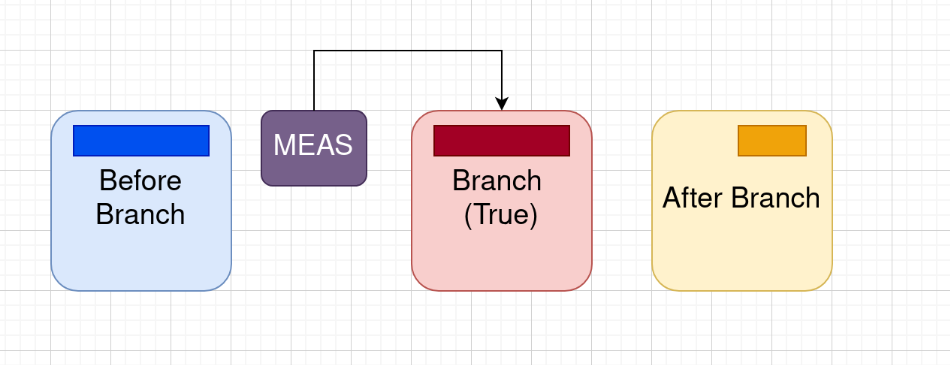
\includegraphics[width=0.6\textwidth]{Images/start.png}
    \caption{Initial configuration of the circuit}
    \label{fig:start}
  \end{figure}

\end{frame}

%---------------------------------------------------------------

\begin{frame}{Novel Pass - Split}

  \begin{itemize}
    \item We first split the \emph{after-branch} subcircuit into parts that are dependent on the measured qubit and those that are not. In other words, the subcircuit \emph{after-branch-1} which is not dependent commutes with the measurement.

      \pause

    \item We also select a certain depth of the \emph{before-branch} subcircuit to combined later. This depth is selected heurstically.
  \end{itemize}

  \pause

  \begin{figure}
    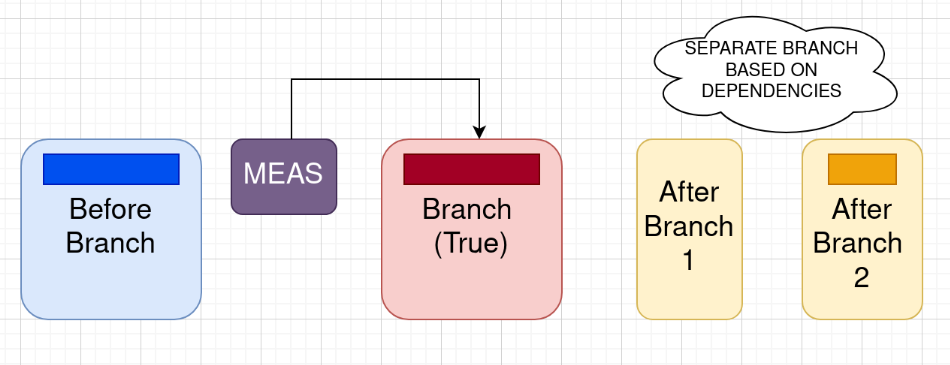
\includegraphics[width=0.6\textwidth]{Images/sep.png}
    \caption{Spliting Phase}
    \label{fig:split}
  \end{figure}

\end{frame}

%---------------------------------------------------------------

\begin{frame}{Novel Pass - Recombine}

  \begin{itemize}
    \item We assume the branch to fail and combine \emph{before-branch} with \emph{after-branch-1}. Note that the measurement result is unchanged and the circuit is still reversible.

      \pause

    \item If our assumption is false, we simply reverse \emph{after-branch-1} and prefix it to the true branch, followed by the remaining \emph{after-branch} subcircuit.

      \pause

    \item Each of the combinations is optimized to the highest degree to reduce the circuit size. In most worst-cases, we recover the original circuit size but do better on average.

      \pause

    \item We can make use of constant-folding to propagate set qubits and cancel gates across the measurement if necessary.
  \end{itemize}

\end{frame}

%---------------------------------------------------------------

\begin{frame}{Novel Pass - Recombine}

  \begin{itemize}
    \item Note that false-branches can also be used but only if it commutes with the measurement. This is a special that may be checked at compile time (although it seems to be expensive).

      \pause

    \item Further recursion is possible with the above assumption but the tradeoff weighs negatively after every recursion.
  \end{itemize}

  \pause

  \begin{figure}
    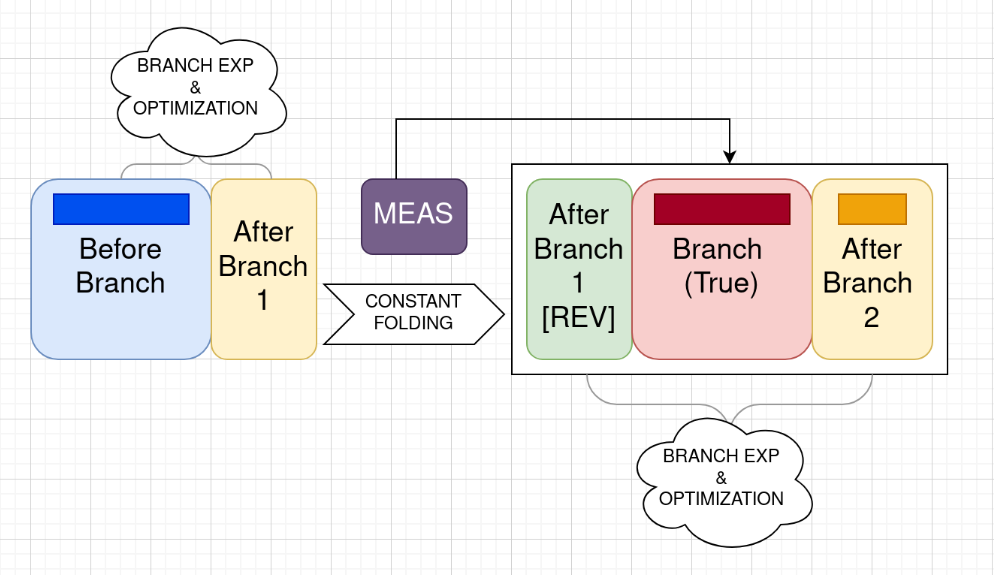
\includegraphics[width=0.6\textwidth]{Images/recomb.png}
    \caption{Recombination Phase}
    \label{fig:recombine}
  \end{figure}


\end{frame}



%%%%%%%%%%%%%%%%%%%%%%%%%%%%%%%%%%%%%%%%%%%%%%%%%%%%%%%%%%%%%%%%%%%

\section{Deliverables \& Timeline}
\begin{frame}{Deliverables}
  \begin{itemize}
    \item (MVP) An investigation on our proposed pass based on the \texttt{Qiskit} transpiler on certain toy examples referenced in bibliography.

    \item (MVP) A simple implementation of the proposed pass on \texttt{Qiskit} transpiler involving \emph{Branch Expansion} and our novel pass.

    \item A MLIR-driven optimization pass for \texttt{cuda-quantum} which will be used to all aforementioned optimizations.
  \end{itemize}
\end{frame}

%---------------------------------------------------------------
\begin{frame}{Timeline \& Contributions}
  \begin{itemize}
    \item \emph{Week 1}:
      \begin{itemize}
        \item Kartheek: Literature reading and investigation/verification of optimizations
        \item Kushagra: Qiskit transpiler overview and sample passes
        \item Rishit: Integrated pseudocode for proposed pass, MLIR pass overview
      \end{itemize}

    \item \emph{Week 2}:
      \begin{itemize}
        \item Kartheek \& Kushagra: Implement Qiskit pass \& experiments
        \item Rishit: Implement MLIR pass
      \end{itemize}

  \end{itemize}
\end{frame}

%---------------------------------------------------------------
% Add your bibliography here
\begin{frame}[allowframebreaks]{References}
  \bibliographystyle{unsrt}
  \bibliography{ref}
\end{frame}



%---------------------------------------------------------------

\end{document}
